\ifdefined\handout
  \documentclass[handout]{beamer}
\else
  \documentclass{beamer}
\fi

\usetheme{boxes}
\usecolortheme{structure}

\setbeamertemplate{footline}[frame number]

\ifdefined\handout
\definecolor{beamer@structure@color}{rgb}{0,0,0}
\setbeamertemplate{navigation symbols}{}
\setbeamercolor{normal text}{fg=black,bg=white}
\setbeamertemplate{frametitle}{\vskip 15pt\color{black}
\def\myhrulefill{\leavevmode\leaders\hrule height 1pt\hfill\kern 0pt}
\headingfont\insertframetitle\par\vskip-8pt\myhrulefill}
\else
\definecolor{beamer@structure@color}{rgb}{1,1,1}
\setbeamertemplate{navigation symbols}{}
\setbeamercolor{normal text}{fg=white,bg=black}
\setbeamertemplate{frametitle}{\vskip 15pt\color{white}
\def\myhrulefill{\leavevmode\leaders\hrule height 1pt\hfill\kern 0pt}
\headingfont\insertframetitle\par\vskip-8pt\myhrulefill}
\fi

\usepackage{amsmath,amssymb}

\newcommand{\NN}{\mathbb{N}}
\newcommand{\ZZ}{\mathbb{Z}}

\DeclareMathOperator{\mcd}{mcd}
\DeclareMathOperator{\mcm}{mcm}

\usepackage[spanish]{babel}

\usepackage{tikz-cd}
\usetikzlibrary{babel}
\usetikzlibrary{calc}

\usepackage{framed}

\newcommand{\dfn}{\mathrel{\mathop:}=}
\newcommand{\rdfn}{=\mathrel{\mathop:}}

\usepackage{mathspec}
\setsansfont[BoldFont={IBM Plex Sans Bold}, ItalicFont={IBM Plex Sans Italic}]{IBM Plex Sans}
\setmonofont[BoldFont={IBM Plex Mono Bold}, ItalicFont={IBM Plex Mono Italic}]{IBM Plex Mono}
\setmathrm[BoldFont={IBM Plex Sans Bold}, ItalicFont={IBM Plex Sans Italic}]{IBM Plex Sans}
\newfontfamily\headingfont[]{IBM Plex Sans Bold}

\setbeamercovered{transparent=10}


\usepackage{array}
\newcolumntype{x}[1]{>{\centering\hspace{0pt}}p{#1}}

\begin{document}

\begin{frame}[plain,noframenumbering]
  \textbf{INTRODUCCIÓN A LA TEORÍA DE NÚMEROS}

  Alexey Beshenov $\mid$ \texttt{cadadr.org}

  \vfill

  \begin{center}\huge\headingfont
    NÚMEROS PRIMOS
  \end{center}

  \vfill
\end{frame}

\begin{frame}
  \frametitle{DEFINICIÓN}

  \begin{itemize}
  \item<2-> Un número natural $p$ es \textbf{primo} si $p \ne 0, 1$ y los únicos
    divisores de $p$ son $\pm 1$ y $\pm p$:
    $$d \mid p \Longrightarrow d = \pm 1 \text{ o } d = \pm p.$$

  \item<3-> Un número natural $a$ es \textbf{compuesto} si $a \ne 0, 1$ y $a$ no
    es primo:
    $$a = bc, \quad 1 < b,c < a.$$

  \item<4-> $1$ es especial y no es ni primo, ni compuesto.

  \item<5-> \textbf{Ejercicio}: si $p$ y $q$ son primos, entonces $p\mid q$
    implica que $p = q$.
  \end{itemize}
\end{frame}

\begin{frame}
  \frametitle{CRITERIO BÁSICO}

  \onslide<2->{\begin{framed}
      $p > 1$ es primo si y solamente si $d \nmid p$ para $1 < d \le \sqrt{p}$.
    \end{framed}}

  \onslide<3->{\textbf{Demostración}.} \onslide<4->{Si $p$ es compuesto,
    entonces
    $$p = ab, \quad 1 < a,b < p.$$}
  \onslide<5->{Necesariamente $a \le \sqrt{p}$ o $b \le \sqrt{p}$. \qed}

  \vspace{1em}

  \onslide<6->{\textbf{Ejemplo}. Es fácil verificar que los primeros primos son
    $$2, 3, 5, 7, 11, 13, 17, 19, 23, 29, \ldots$$}
\end{frame}

\begin{frame}
  \frametitle{TODO NÚMERO TIENE UN DIVISOR PRIMO}

  \onslide<2->{\begin{framed}
      \textbf{Lema}. Para todo $a > 1$ existe un divisor primo $p \mid a$.
    \end{framed}}

  \onslide<3->{\textbf{Demostración}.}

  \begin{itemize}
  \item<4-> Si $a$ es primo, $p = a$.

  \item<5-> Sino, existe un divisor no trivial $d \mid a$ tal que $1 < d < a$.

    Si $d$ es primo, $p = d$.

  \item<6-> Sino, existe un divisor no trivial $d_1 \mid d$, etc.
  \end{itemize}

  \onslide<7->{\[
      \cdots \mid d_2 \mid d_1 \mid d \mid a,
      \quad
      \cdots < d_2 < d_1 < d < a.
    \]}

  \onslide<8->{Los $d_i > 1$ decrecen, así que en algún momento el proceso
    termina. \qed}
\end{frame}

\begin{frame}
  \frametitle{TODO NÚMERO SE DESCOMPONE EN PRIMOS}

  \onslide<2->{\begin{framed}
      Todo $a > 1$ puede ser escrito como $a = p_1 \cdots p_s$, donde los $p_i$
      son primos (no necesariamente distintos).
    \end{framed}}

  \onslide<3->{\textbf{Demostración}.}

  \begin{itemize}
  \item<4-> Existe un divisor primo $p_1 \mid a$.

  \item<5-> Si $a \ne p_1$, ponemos $a_2 = a/p_1$ y tomamos $p_2 \mid a_2$.

  \item<6-> Pasamos a $a_3 = a_2/p_2$, etc.

  \item<7-> Los $a_i$ decrecen, y el proceso termina. \qed
  \end{itemize}
\end{frame}

\begin{frame}
  \frametitle{EJEMPLO}

  \begin{itemize}
  \item<2-> $a = 420$ es par, podemos dividirlo por $p_1 = 2$.

  \item<3-> $a_1 = 420/2 = 210$ es también par, $p_2 = 2$.

  \item<4-> $a_2 = 210/2 = 105$ es divisible por $p_3 = 3$.

  \item<5-> $a_3 = 105/3 = 35$ es divisible por $p_4 = 5$.

  \item<6-> $a_4 = 35/5 = 7$ es primo. $p_5 = 7$.
  \end{itemize}

  \onslide<7->{\[
      420 = 2\cdot 2\cdot 3\cdot 5\cdot 7.
    \]}

  \onslide<8->{¿Habrá otra descomposición en primos?}
\end{frame}

\begin{frame}
  \frametitle{EL TEOREMA FUNDAMENTAL DE LA ARITMÉTICA}

  \begin{itemize}
  \item<2-> Más o menos inmediato de la definición:

    descomposición en primos $a = p_1 \cdots p_s$.

  \item<3-> Parece obvio, pero no lo es:

    los $p_i$ son únicos, salvo permutación de los múltiplos.

  \item<4-> Necesitamos más preparación para probarlo.
  \end{itemize}
\end{frame}

\begin{frame}
  \frametitle{INFINITUD DE PRIMOS}

  \onslide<2->{\begin{framed}
      \textbf{Teorema (Euclides)}. Existen infinitos números primos.
    \end{framed}}

  \onslide<3->{\textbf{Demostración}.}

  \begin{itemize}
  \item<4-> Sean $p_1, \ldots, p_k$ primos.

  \item<5-> Consideremos $a = p_1 \cdots p_k + 1$.

    $p_i \nmid a$ para $i = 1,\ldots,k$ (el residuo es $1$).

  \item<6-> $p \mid a$ para algún primo $p$, así que $p \ne p_1, \ldots, p_k$. \qed
  \end{itemize}

  \vspace{1em}

  \onslide<7->{* No es una manera muy práctica de generar primos.}
\end{frame}

\begin{frame}
  \frametitle{EJEMPLO}

  \begin{align*}
    \onslide<2->{p_1} & \onslide<2->{= 2,} \\
    \onslide<3->{p_2} & \onslide<3->{= p_1 + 1 = 3,} \\
    \onslide<4->{p_3} & \onslide<4->{= p_1\,p_2 + 1 = 7,} \\
    \onslide<5->{p_4} & \onslide<5->{= p_1\,p_2\,p_3 + 1 = 43;}
  \end{align*}

  \onslide<6->{\begin{gather*}
      p_1\,p_2\,p_3\,p_4 + 1 = 1807 = 13\cdot 139 \quad \text{compuesto}, \\
      p_5 = 13;
    \end{gather*}}

  \onslide<7->{\begin{gather*}
      p_1\,p_2\,p_3\,p_4\,p_5 + 1 = 23479 = 53\cdot 443 \quad \text{compuesto}, \\
      p_6 = 53, \quad \text{etc.}
  \end{gather*}}
\end{frame}

\begin{frame}
  \frametitle{CRIBA DE ERATÓSTENES}

  \begin{center}\small
    \renewcommand{\arraystretch}{1.6}
    \begin{tabular}{x{0.65cm}x{0.65cm}x{0.65cm}x{0.65cm}x{0.65cm}x{0.65cm}x{0.65cm}x{0.65cm}x{0.65cm}x{0.65cm}}
\onslide<1>{$1$} & $2$ & $3$ & \onslide<-2>{$4$} & $5$ & \onslide<-2>{$6$} & $7$ & \onslide<-2>{$8$} & \onslide<-3>{$9$} & \onslide<-2>{$10$} \tabularnewline
$11$ & \onslide<-2>{$12$} & $13$ & \onslide<-2>{$14$} & \onslide<-3>{$15$} & \onslide<-2>{$16$} & $17$ & \onslide<-2>{$18$} & $19$ & \onslide<-2>{$20$} \tabularnewline
\onslide<-3>{$21$} & \onslide<-2>{$22$} & $23$ & \onslide<-2>{$24$} & \onslide<-4>{$25$} & \onslide<-2>{$26$} & \onslide<-3>{$27$} & \onslide<-2>{$28$} & $29$ & \onslide<-2>{$30$} \tabularnewline
$31$ & \onslide<-2>{$32$} & \onslide<-3>{$33$} & \onslide<-2>{$34$} & \onslide<-4>{$35$} & \onslide<-2>{$36$} & $37$ & \onslide<-2>{$38$} & \onslide<-3>{$39$} & \onslide<-2>{$40$} \tabularnewline
$41$ & \onslide<-2>{$42$} & $43$ & \onslide<-2>{$44$} & \onslide<-3>{$45$} & \onslide<-2>{$46$} & $47$ & \onslide<-2>{$48$} & \onslide<-5>{$49$} & \onslide<-2>{$50$} \tabularnewline
\onslide<-3>{$51$} & \onslide<-2>{$52$} & $53$ & \onslide<-2>{$54$} & \onslide<-4>{$55$} & \onslide<-2>{$56$} & \onslide<-3>{$57$} & \onslide<-2>{$58$} & $59$ & \onslide<-2>{$60$} \tabularnewline
$61$ & \onslide<-2>{$62$} & \onslide<-3>{$63$} & \onslide<-2>{$64$} & \onslide<-4>{$65$} & \onslide<-2>{$66$} & $67$ & \onslide<-2>{$68$} & \onslide<-3>{$69$} & \onslide<-2>{$70$} \tabularnewline
$71$ & \onslide<-2>{$72$} & $73$ & \onslide<-2>{$74$} & \onslide<-3>{$75$} & \onslide<-2>{$76$} & \onslide<-5>{$77$} & \onslide<-2>{$78$} & $79$ & \onslide<-2>{$80$} \tabularnewline
\onslide<-3>{$81$} & \onslide<-2>{$82$} & $83$ & \onslide<-2>{$84$} & \onslide<-4>{$85$} & \onslide<-2>{$86$} & \onslide<-3>{$87$} & \onslide<-2>{$88$} & $89$ & \onslide<-2>{$90$} \tabularnewline
\onslide<-5>{$91$} & \onslide<-2>{$92$} & \onslide<-3>{$93$} & \onslide<-2>{$94$} & \onslide<-4>{$95$} & \onslide<-2>{$96$} & $97$ & \onslide<-2>{$98$} & \onslide<-3>{$99$} & \onslide<-2>{$100$} \tabularnewline
    \end{tabular}
  \end{center}

  \onslide<6->{~}
\end{frame}
  
\begin{frame}
  \frametitle{CONCLUSIÓN}

  \onslide<2->{Los primos $p < 100$ son
    \begin{gather*}
      2, 3, 5, 7, 11,
      13, 17, 19, 23, 29, \\
      31, 37, 41, 43, 47,
      53, 59, 61, 67, 71, \\
      73, 79, 83, 89, 97.
    \end{gather*}}

  \onslide<3->{\textbf{Ejercicio}. Determine con la criba cuáles son los primos $p < 200$ (hay $46$ de estos).}
\end{frame}

\begin{frame}
  \frametitle{ERATÓSTENES}

  \begin{center}
    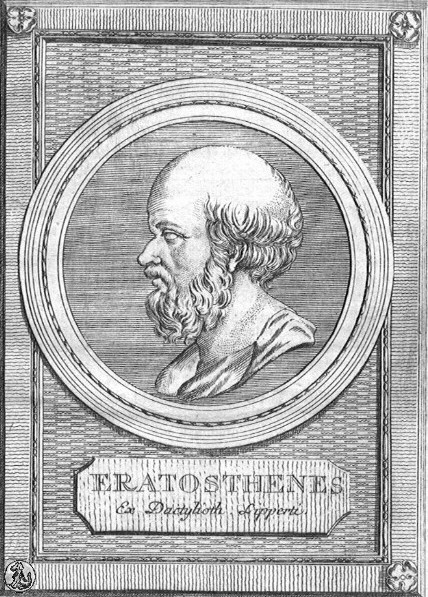
\includegraphics[width=0.35\textwidth]{eratosthenes.jpg}

    Eratóstenes de Cirene

    (276--194 a.C.)
  \end{center}
\end{frame}

\begin{frame}[plain,noframenumbering]

  \vfill

  \begin{center}\huge\headingfont
    EJERCICIOS
  \end{center}

  \vfill
\end{frame}

\begin{frame}
  \frametitle{EJERCICIO 1: PRIMOS DE LA FORMA $11\cdots 1$}

  \onslide<2->{Los números
    \[
      11, ~
      \underbrace{1111111111111111111}_{19\text{ unos}}, ~
      \underbrace{11111111111111111111111}_{23\text{ unos}}
    \]
    son primos.}

  \onslide<3->{Demuestre que en cualquier base $b$, si
    $\underline{11\cdots 1}_b$ es primo, entonces el número de unos es también
    primo.}

  \onslide<4->{\textbf{Ejemplo}.}
  \onslide<5->{\begin{align*}
    \underline{111}_3 & = 13, \\
    \underline{111}_5 & = 31, \\
    \underline{11111}_2 & = 31, \\
    \underline{11111}_7 & = 2801, \\
    \underline{11111111111}_5 & = 12207031, \\
    \underline{11111111111}_{17} & = 2141993519227, \\
                      & \ldots
  \end{align*}}
\end{frame}

\begin{frame}
  \frametitle{EJERCICIO 2: POLINOMIOS CON VALORES PRIMOS}

  \begin{itemize}
  \item<2-> Encuentre el más pequeño $a > 0$ tal que $a^4 + (a+1)^4$ es
    compuesto.

  \item<3-> Encuentre el más pequeño $a > 0$ tal que $a^2 - a + 11$ es
    compuesto.

  \item<4-> Euler: $a^2 - a + 41$ toma valores primos para $a = 1, \ldots, 40$.
  \end{itemize}
\end{frame}

\begin{frame}
  \frametitle{EJERCICIO 3: PRIMOS DE LA FORMA $a^n + 1$}

  \onslide<2->{Demuestre que si $a^n + 1$ es primo para $a > 1$, entonces $a$ es
    par y $n = 2^k$ es una potencia de $2$.}

  \onslide<3->{\textbf{Ejemplo}.}

  \onslide<4->{\begin{align*}
    2^2 + 1 & = 5, \\
    2^4 + 1 & = 17, \\ 
    6^2 + 1 & = 37, \\
    10^2 + 1 & = 101, \\
    14^2 + 1 & = 197, \\
    2^8 + 1 & = 257, \\
    20^2 + 1 & = 401, \\
            & \cdots
  \end{align*}}
\end{frame}

\begin{frame}
  \frametitle{PRIMOS DE FERMAT: $2^{2^k} + 1$}

  \begin{minipage}[t][0.6\textheight]{0.6\textwidth}
    \begin{align*}
      \onslide<2->{2^{2^0} + 1} & \onslide<2->{= 3,} \\
      \onslide<3->{2^{2^1} + 1} & \onslide<3->{= 5,} \\
      \onslide<4->{2^{2^2} + 1} & \onslide<4->{= 17,} \\
      \onslide<5->{2^{2^3} + 1} & \onslide<5->{= 257,} \\
      \onslide<6->{2^{2^4} + 1} & \onslide<6->{= 65537.} \\
    \end{align*}
  \end{minipage}
  \begin{minipage}[t]{0.35\textwidth}
    \vspace{0pt}\flushright
    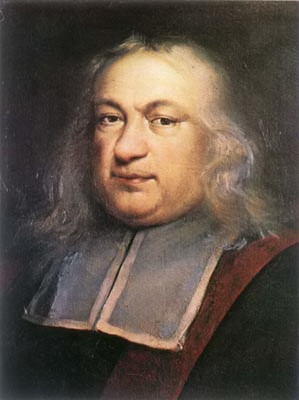
\includegraphics[width=.9\textwidth]{fermat.jpg}

    Pierre de Fermat\\
    (1601--1665)
  \end{minipage}
\end{frame}

\begin{frame}
  \frametitle{¿SON PRIMOS LOS PRIMOS DE FERMAT?}

  \begin{itemize}
  \item<2-> Euler: $641 \mid (2^{2^5} + 1)$.

    \[ 2^{2^5} + 1 = 641\cdot 6700417. \]

  \item<3-> $2^{2^6} + 1 = 274177\cdot 67280421310721$.

  \item<4-> $2^{2^7} + 1 = 59649589127497217\cdot 5704689200685129054721$.

  \item<5-> \dots

  \item<6-> Aún no se conoce ningún $k > 4$ tal que $2^{2^k} + 1$ sea primo.
  \end{itemize}
\end{frame}

\begin{frame}[plain,noframenumbering]

  \vfill

  \begin{center}\huge\headingfont
    ¡GRACIAS POR SU ATENCIÓN!
  \end{center}

  \vfill
\end{frame}
\end{document}
